

\subsection{Parzen window classification}


\begin{frame}\frametitle{\subsecname}

Prediction is based on 
\begin{itemize}
\item \underline{all} data points \notesonly{(no longer restricted to the $k$ nearest neighbors)}
\item \notesonly{and the contribution of each point is} weighted according to some window/``kernel'' function $\kappa(\vec x, \vec x')$ \notesonly{evaluated for a pair of points $\vec x$ and $\vec x'$}.
\end{itemize}

\begin{equation}
\vec y(\vec x) := \frac{1}{Z} \sum_{\alpha=1}^{p}\;\vec y_T^{(\alpha)} \kappa(\vec x, \vec x^{(\alpha)})
\end{equation}

with

\begin{equation}
Z := \sum_{\alpha=1}^{p} \kappa(\vec x, \vec x^{(\alpha)})
\end{equation}

\end{frame}

\begin{frame}

An example for the window/``kernel'' function $\kappa(\vec x, \vec x')$ would be the Gaussian function:

\begin{equation}
\kappa(\vec x, \vec x') := \exp\left( -\,\frac{\lVert \vec x - \vec x'\rVert^2_2}{2\,\sigma_{\kappa}^2} \right)
\label{eq:gauss_kernel}
\end{equation}

where $\sigma_{\kappa}$ is referred to as the \emph{width} of the kernel.

\begin{figure}[ht]
     \centering
     \savebox{\imagebox}{
	 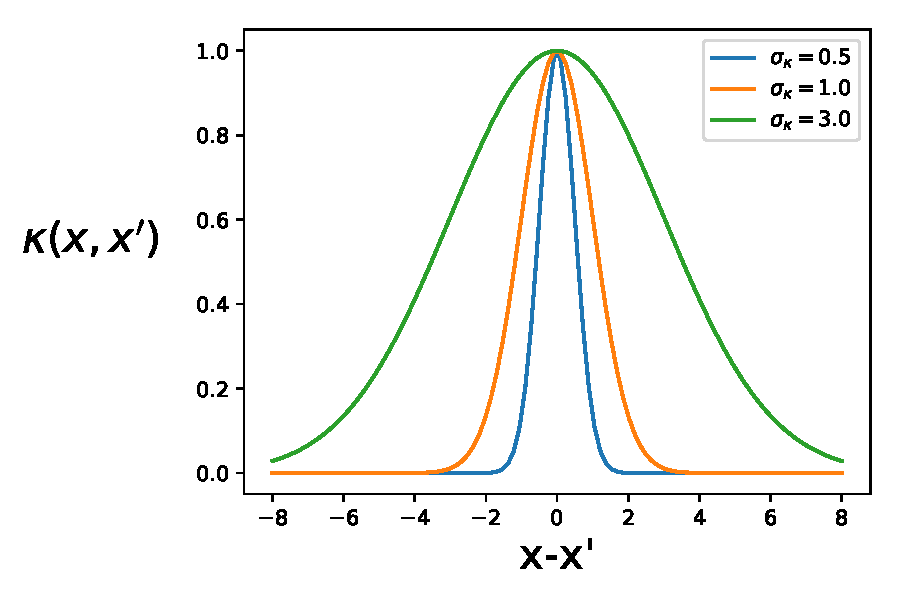
\includegraphics[width=0.45\textwidth]{img/guassian_function_1d}}%
     \begin{subfigure}[t]{0.45\textwidth}
         \centering
         \usebox{\imagebox}% Place largest image
         \caption{For data in 1D}
         \label{fig:quadratic}
     \end{subfigure}
     \hspace{2mm}
     \begin{subfigure}[t]{0.45\textwidth}
         \centering
         \raisebox{\dimexpr.5\ht\imagebox-.5\height}{% Raise smaller image into place
         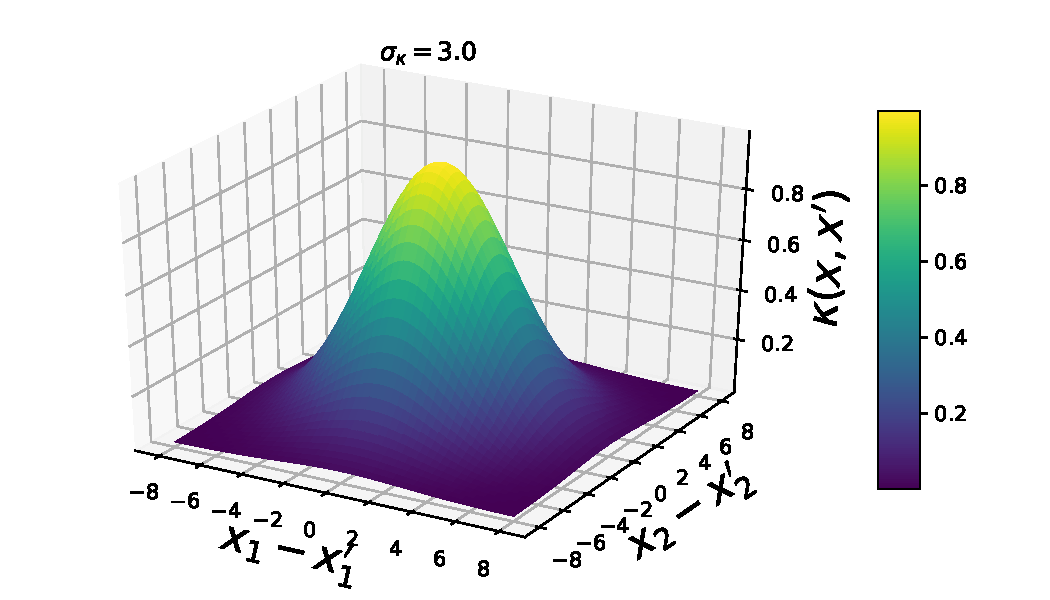
\includegraphics[width=0.99\textwidth]{img/guassian_function_2d_3Dview}
         }
         \caption{For data in 2D}
         \label{fig:linear}
     \end{subfigure}
     \mode<article>{
     \caption{The Gaussian kernel function}
     }
	 \label{fig:quadratic_density_gaussian}
\end{figure}

\end{frame}

\begin{frame}

Binary classification example with 2D data:

\begin{figure}[ht]
     \centering
     \savebox{\imagebox}{
	 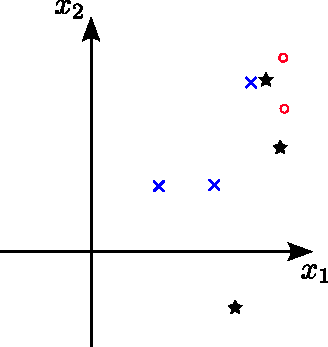
\includegraphics[width=0.3\textwidth]{img/parzen_data}}%
     \begin{subfigure}[t]{0.3\textwidth}
         \centering
         \usebox{\imagebox}% Place largest image
         \caption{For data in 1D}
         \label{fig:quadratic}
     \end{subfigure}
     \hspace{2mm}
     \visible<2>{
     \begin{subfigure}[t]{0.3\textwidth}
         \centering
         \raisebox{\dimexpr.5\ht\imagebox-.5\height}{% Raise smaller image into place
         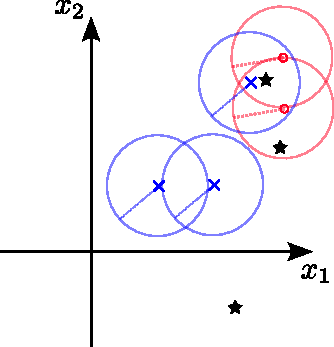
\includegraphics[width=0.99\textwidth]{img/parzen_circles}
         }
         \caption{For data in 2D}
         \label{fig:linear}
     \end{subfigure}
     }
\end{figure}


\mode<presentation>{

\begin{equation}
\vec y(\vec x) := \frac{1}{Z} \sum_{\alpha=1}^{p} \vec y_T^{(\alpha)} \, \kappa(\vec x, \vec x^{(\alpha)})
\end{equation}

\begin{equation}
\kappa(\vec x, \vec x^{(\alpha)}) := \exp\left( -\,\frac{\lVert \vec x - \vec x^{(\alpha)}\rVert^2_2}{2\,\sigma_{\kappa}^2} \right)
\label{eq:gauss_kernel}
\end{equation}

}

\end{frame}

\begin{frame}

\begin{figure}[ht]
     \centering
     \savebox{\imagebox}{
	 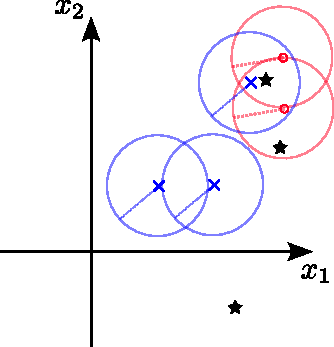
\includegraphics[width=0.37\textwidth]{img/parzen_circles}}%
     \begin{subfigure}[t]{0.37\textwidth}
         \centering
         \usebox{\imagebox}% Place largest image
         \caption{wide kernel width}
         \label{fig:quadratic}
     \end{subfigure}
     \hspace{2mm}
     \begin{subfigure}[t]{0.37\textwidth}
         \centering
         \raisebox{\dimexpr.5\ht\imagebox-.5\height}{% Raise smaller image into place
         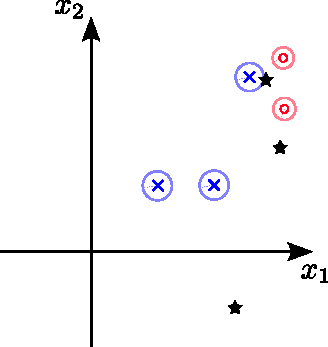
\includegraphics[width=0.99\textwidth]{img/parzen_circles_narrow}
         }
         \caption{narrow kernel width}
         \label{fig:linear}
     \end{subfigure}
\end{figure}

\question{What is the role of the kernel width $\sigma_{\kappa}$ in terms of model complexity?}

\pause

Hint: Jitter the query points (or the data) and see which choice of $\sigma_{\kappa}$ will lead to different (more noisy) predictions.

\end{frame}

\begin{frame}

Remarks:
\begin{enumerate} 
\item The width of the kernel $\kappa$ controls the model complexity (narrow width $\leadsto$ over-fitting (high variance), wide $\leadsto$ under-fitting)
 
One way to go about this is to apply a small noise to the query points (i.e. jitter) and see how the predictions will vary with different $\sigma_{\kappa}$. If this small noise in the position of the points leads to different predictions we are basically looking at high variance.

\item Using all data points. Potentially costly with large $p$
\end{enumerate}
\end{frame}
